%% WealthPilot Pro - Portfolio Analysis Report
%% Generated: December 24, 2025
%% LaTeX Code - Compile with pdflatex

\documentclass[11pt,a4paper]{article}

% Packages
\usepackage[utf8]{inputenc}
\usepackage[T1]{fontenc}
\usepackage{lmodern}
\usepackage[margin=1in]{geometry}
\usepackage{graphicx}
\usepackage{xcolor}
\usepackage{tikz}
\usepackage{pgfplots}
\usepackage{booktabs}
\usepackage{longtable}
\usepackage{fancyhdr}
\usepackage{titlesec}
\usepackage{hyperref}
\usepackage{fontawesome5}
\usepackage{tcolorbox}
\usepackage{colortbl}
\usepackage{array}
\usepackage{multirow}

\pgfplotsset{compat=1.18}
\usetikzlibrary{patterns,shadows,positioning,calc}

% Colors
\definecolor{primary}{HTML}{0F172A}
\definecolor{secondary}{HTML}{1E40AF}
\definecolor{accent}{HTML}{3B82F6}
\definecolor{success}{HTML}{059669}
\definecolor{danger}{HTML}{DC2626}
\definecolor{warning}{HTML}{D97706}
\definecolor{lightbg}{HTML}{F8FAFC}
\definecolor{border}{HTML}{E5E7EB}

% Page style
\pagestyle{fancy}
\fancyhf{}
\fancyhead[L]{\textcolor{primary}{\textbf{WealthPilot Pro}}}
\fancyhead[R]{\textcolor{gray}{Portfolio Analysis Report}}
\fancyfoot[C]{\textcolor{gray}{Page \thepage}}
\renewcommand{\headrulewidth}{0.5pt}

% Title formatting
\titleformat{\section}{\Large\bfseries\color{primary}}{\thesection}{1em}{}[\titlerule]
\titleformat{\subsection}{\large\bfseries\color{secondary}}{\thesubsection}{1em}{}

\begin{document}

% ============================================================
% COVER PAGE
% ============================================================
\begin{titlepage}
\centering
\vspace*{2cm}

{\Huge\bfseries\textcolor{primary}{WealthPilot Pro}}\\[0.5cm]
{\Large\textcolor{secondary}{AI-Powered Portfolio Intelligence}}\\[2cm]


\begin{tikzpicture}
\draw[primary, line width=2pt] (0,0) -- (12,0);
\end{tikzpicture}\\[1cm]

{\LARGE\bfseries Portfolio Analysis Report}\\[0.5cm]
{\Large Diversified Growth \& Income Portfolio}\\[1cm]

{\large December 24, 2025}\\[2cm]

\begin{tcolorbox}[colback=lightbg,colframe=border,width=0.8\textwidth,arc=3mm]
\centering
\begin{tabular}{cc}
\textbf{Total Portfolio Value} & \textbf{Total Return} \\[0.3cm]
{\LARGE\textcolor{primary}{\$324,715}} &
{\LARGE\textcolor{success}{+25.23\%}} \\[0.5cm]
\textbf{Holdings} & \textbf{Dividend Yield} \\[0.3cm]
{\LARGE\textcolor{primary}{22}} &
{\LARGE\textcolor{secondary}{1.12\%}} \\
\end{tabular}
\end{tcolorbox}

\vfill
{\small\textcolor{gray}{Powered by AI Analysis $\bullet$ For Informational Purposes Only}}
\end{titlepage}

% ============================================================
% EXECUTIVE SUMMARY
% ============================================================
\section{Executive Summary}

\begin{tcolorbox}[colback=green!70!black!10,colframe=green!70!black,title={\textbf{Portfolio Health: EXCELLENT}},fonttitle=\large\bfseries]
Your portfolio has delivered a total return of \textbf{+25.23\%} with \textbf{73\%} of positions profitable. The portfolio contains 22 holdings across 8 sectors.
\end{tcolorbox}

\subsection{Key Metrics}

\begin{center}
\begin{tabular}{|l|r|}
\hline
\rowcolor{primary!10}
\textbf{Metric} & \textbf{Value} \\
\hline
Total Portfolio Value & \$324,715 \\
Total Cost Basis & \$259,300 \\
Total Gain/Loss & \$65,415 (+25.23\%) \\
Win Rate & 72.7\% (16/22 positions) \\
Portfolio Yield & 1.12\% \\
Annual Dividend Income & \$3,622.967 \\
\hline
\end{tabular}
\end{center}

% ============================================================
% PORTFOLIO ALLOCATION
% ============================================================
\section{Portfolio Allocation}

\subsection{Sector Breakdown}

\begin{center}
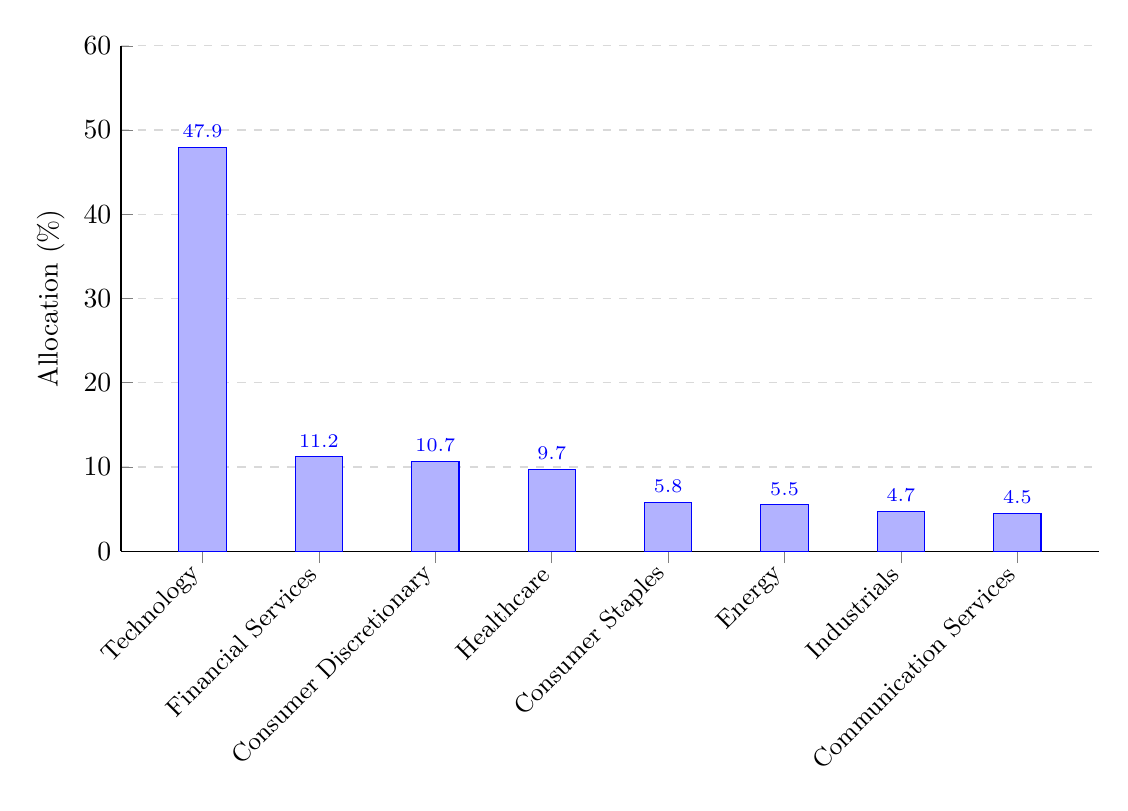
\begin{tikzpicture}
\begin{axis}[
    ybar,
    width=14cm,
    height=8cm,
    bar width=0.6cm,
    ylabel={Allocation (\%)},
    symbolic x coords={Technology,Financial Services,Consumer Discretionary,Healthcare,Consumer Staples,Energy,Industrials,Communication Services},
    xtick=data,
    x tick label style={rotate=45,anchor=east,font=\small},
    ymin=0,
    ymax=60,
    nodes near coords,
    nodes near coords style={font=\scriptsize},
    every axis plot/.append style={fill=accent!70},
    axis lines*=left,
    ymajorgrids=true,
    grid style={dashed,gray!30},
]
\addplot coordinates {(Technology,47.9) (Financial Services,11.2) (Consumer Discretionary,10.7) (Healthcare,9.7) (Consumer Staples,5.8) (Energy,5.5) (Industrials,4.7) (Communication Services,4.5)};
\end{axis}
\end{tikzpicture}
\end{center}

\subsection{Top 10 Holdings}

\begin{center}
\begin{tabular}{|c|l|r|r|r|r|}
\hline
\rowcolor{primary!10}
\textbf{\#} & \textbf{Symbol} & \textbf{Value} & \textbf{Weight} & \textbf{Return} & \textbf{Sector} \\
\hline
1 & MSFT & \$45,360 & 14.0\% & \textcolor{success}{+35.00\%} & Technology \\\hline
2 & NVDA & \$39,600 & 12.2\% & \textcolor{success}{+98.00\%} & Technology \\\hline
3 & AAPL & \$38,700 & 11.9\% & \textcolor{success}{+33.45\%} & Technology \\\hline
4 & META & \$17,900 & 5.5\% & \textcolor{success}{+98.89\%} & Technology \\\hline
5 & AMZN & \$16,020 & 4.9\% & \textcolor{success}{+36.92\%} & Consumer Discre \\\hline
6 & GOOGL & \$14,100 & 4.3\% & \textcolor{success}{+17.50\%} & Technology \\\hline
7 & JPM & \$13,860 & 4.3\% & \textcolor{success}{+41.43\%} & Financial Servi \\\hline
8 & UNH & \$13,200 & 4.1\% & \textcolor{success}{+1.54\%} & Healthcare \\\hline
9 & JNJ & \$12,480 & 3.8\% & \textcolor{danger}{-5.45\%} & Healthcare \\\hline
10 & V & \$11,790 & 3.6\% & \textcolor{success}{+19.09\%} & Financial Servi \\\hline
\end{tabular}
\end{center}

% ============================================================
% PERFORMANCE ANALYSIS
% ============================================================
\section{Performance Analysis}

\subsection{Benchmark Comparison}

\begin{center}
\begin{tabular}{|l|r|r|r|}
\hline
\rowcolor{primary!10}
\textbf{Index} & \textbf{Return} & \textbf{Your Portfolio} & \textbf{Difference} \\
\hline
S\&P 500 & +12.50\% & +25.23\% & +12.73\% \\
NASDAQ & +15.20\% & +25.23\% & +10.03\% \\
Dow Jones & +10.80\% & +25.23\% & +14.43\% \\
\hline
\end{tabular}
\end{center}

\subsection{Top Performers}

\begin{center}
\begin{tabular}{|l|r|r|}
\hline
\rowcolor{success!20}
\textbf{Symbol} & \textbf{Return} & \textbf{Gain} \\
\hline
META & \textcolor{success}{+98.89\%} & \$8,900 \\\hline
NVDA & \textcolor{success}{+98.00\%} & \$19,600 \\\hline
JPM & \textcolor{success}{+41.43\%} & \$4,060 \\\hline
NFLX & \textcolor{success}{+38.57\%} & \$2,025 \\\hline
AMZN & \textcolor{success}{+36.92\%} & \$4,320 \\\hline
\end{tabular}
\end{center}

\subsection{Underperformers}

\begin{center}
\begin{tabular}{|l|r|r|}
\hline
\rowcolor{danger!20}
\textbf{Symbol} & \textbf{Return} & \textbf{Loss} \\
\hline
PFE & \textcolor{danger}{-32.14\%} & \$-2,700 \\\hline
DIS & \textcolor{danger}{-16.36\%} & \$-1,440 \\\hline
UPS & \textcolor{danger}{-12.22\%} & \$-880 \\\hline
TSLA & \textcolor{danger}{-10.00\%} & \$-1,120 \\\hline
JNJ & \textcolor{danger}{-5.45\%} & \$-720 \\\hline
\end{tabular}
\end{center}

% ============================================================
% RISK ASSESSMENT
% ============================================================
\section{Risk Assessment}

\begin{tcolorbox}[colback=lightbg,colframe=primary,title={\textbf{Risk Score: 6/10 (Moderate)}},fonttitle=\large\bfseries]
\begin{itemize}
\item \textbf{Concentration Risk:} MEDIUM - Top 5 holdings represent 48.5\% of portfolio
\item \textbf{Sector Risk:} HIGH - Technology at 47.9\%
\item \textbf{Diversification Score:} 29/100
\item \textbf{HHI Index:} 707 (lower is more diversified)
\end{itemize}
\end{tcolorbox}

% ============================================================
% COMPLETE HOLDINGS
% ============================================================
\section{Complete Holdings Detail}

\begin{center}
\small
\begin{longtable}{|c|l|r|r|r|r|r|l|}
\hline
\rowcolor{primary!10}
\textbf{\#} & \textbf{Symbol} & \textbf{Shares} & \textbf{Avg Cost} & \textbf{Price} & \textbf{Value} & \textbf{Return} & \textbf{Sector} \\
\hline
\endhead
1 & MSFT & 120.00 & \$280.00 & \$378.00 & \$45,360 & \textcolor{success}{+35.00\%} & Technology \\\hline
2 & NVDA & 80.00 & \$250.00 & \$495.00 & \$39,600 & \textcolor{success}{+98.00\%} & Technology \\\hline
3 & AAPL & 200.00 & \$145.00 & \$193.50 & \$38,700 & \textcolor{success}{+33.45\%} & Technology \\\hline
4 & META & 50.00 & \$180.00 & \$358.00 & \$17,900 & \textcolor{success}{+98.89\%} & Technology \\\hline
5 & AMZN & 90.00 & \$130.00 & \$178.00 & \$16,020 & \textcolor{success}{+36.92\%} & Consumer Dis \\\hline
6 & GOOGL & 100.00 & \$120.00 & \$141.00 & \$14,100 & \textcolor{success}{+17.50\%} & Technology \\\hline
7 & JPM & 70.00 & \$140.00 & \$198.00 & \$13,860 & \textcolor{success}{+41.43\%} & Financial Se \\\hline
8 & UNH & 25.00 & \$520.00 & \$528.00 & \$13,200 & \textcolor{success}{+1.54\%} & Healthcare \\\hline
9 & JNJ & 80.00 & \$165.00 & \$156.00 & \$12,480 & \textcolor{danger}{-5.45\%} & Healthcare \\\hline
10 & V & 45.00 & \$220.00 & \$262.00 & \$11,790 & \textcolor{success}{+19.09\%} & Financial Se \\\hline
11 & BRK.B & 30.00 & \$320.00 & \$358.00 & \$10,740 & \textcolor{success}{+11.88\%} & Financial Se \\\hline
12 & XOM & 100.00 & \$85.00 & \$105.00 & \$10,500 & \textcolor{success}{+23.53\%} & Energy \\\hline
13 & TSLA & 40.00 & \$280.00 & \$252.00 & \$10,080 & \textcolor{danger}{-10.00\%} & Consumer Dis \\\hline
14 & PG & 60.00 & \$145.00 & \$158.00 & \$9,480 & \textcolor{success}{+8.97\%} & Consumer Sta \\\hline
15 & KO & 150.00 & \$55.00 & \$62.00 & \$9,300 & \textcolor{success}{+12.73\%} & Consumer Sta \\\hline
16 & CAT & 30.00 & \$240.00 & \$295.00 & \$8,850 & \textcolor{success}{+22.92\%} & Industrials \\\hline
17 & HD & 25.00 & \$300.00 & \$348.00 & \$8,700 & \textcolor{success}{+16.00\%} & Consumer Dis \\\hline
18 & CVX & 50.00 & \$150.00 & \$148.00 & \$7,400 & \textcolor{danger}{-1.33\%} & Energy \\\hline
19 & DIS & 80.00 & \$110.00 & \$92.00 & \$7,360 & \textcolor{danger}{-16.36\%} & Communicatio \\\hline
20 & NFLX & 15.00 & \$350.00 & \$485.00 & \$7,275 & \textcolor{success}{+38.57\%} & Communicatio \\\hline
21 & UPS & 40.00 & \$180.00 & \$158.00 & \$6,320 & \textcolor{danger}{-12.22\%} & Industrials \\\hline
22 & PFE & 200.00 & \$42.00 & \$28.50 & \$5,700 & \textcolor{danger}{-32.14\%} & Healthcare \\\hline
\hline
\rowcolor{primary!20}
\multicolumn{5}{|r|}{\textbf{TOTAL}} & \textbf{\$324,715} & \textbf{+25.23\%} & \\
\hline
\end{longtable}
\end{center}

% ============================================================
% DIVIDEND ANALYSIS
% ============================================================
\section{Dividend Analysis}

\subsection{Income Summary}

\begin{center}
\begin{tabular}{|l|r|}
\hline
\rowcolor{secondary!10}
\textbf{Metric} & \textbf{Value} \\
\hline
Annual Dividend Income & \$3,622.967 \\
Portfolio Yield & 1.12\% \\
Monthly Income & \$301.914 \\
Quarterly Income & \$905.742 \\
Dividend-Paying Holdings & 15 of 22 \\
\hline
\end{tabular}
\end{center}

% ============================================================
% RECOMMENDATIONS
% ============================================================
\section{Recommendations}

\begin{tcolorbox}[colback=accent!5,colframe=accent,title={\textbf{Action Items}},fonttitle=\large\bfseries]
\begin{enumerate}
\item \textbf{Concentration:} Position sizing is acceptable
\item \textbf{Sector Rebalancing:} Reduce Technology exposure below 30\%
\item \textbf{Diversification:} Position count is adequate
\item \textbf{Take Profits:} Consider trimming positions with >50\% gains
\end{enumerate}
\end{tcolorbox}

% ============================================================
% DISCLAIMER
% ============================================================
\section*{Important Disclaimer}

\begin{tcolorbox}[colback=warning!10,colframe=warning]
\small
This report is generated by WealthPilot Pro for \textbf{informational purposes only}. It does not constitute financial advice, investment recommendations, or an offer to buy or sell securities.

\textbf{Past performance is not indicative of future results.} All investments involve risk, including the potential loss of principal. Before making investment decisions, consult with a qualified financial advisor.

\vspace{0.3cm}
\textit{Report generated: December 24, 2025}
\end{tcolorbox}

\end{document}
